\section{Parking Lot Generation}

Once the plot generation is finished the parking lot generation starts to fill some of the generated plots with parking lots.
The generated parking lots consist of one or more rows of parking spaces (see Figure~\ref{fig:results_parking_sizebased}).

\begin{figure}[H]
   \centering
   \begin{subfigure}[b]{0.38\textwidth}
     \frame{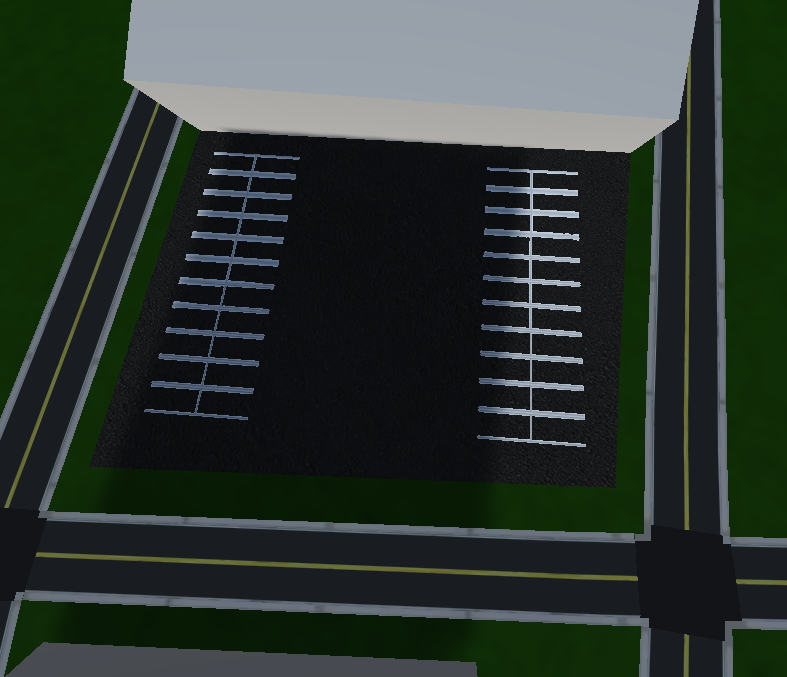
\includegraphics[width=\textwidth]{figure/results/parking/bigplot}}
     \caption{Large parking lot consisting of two rows.}
   \end{subfigure}
   \quad
   \begin{subfigure}[b]{0.52\textwidth}
     \frame{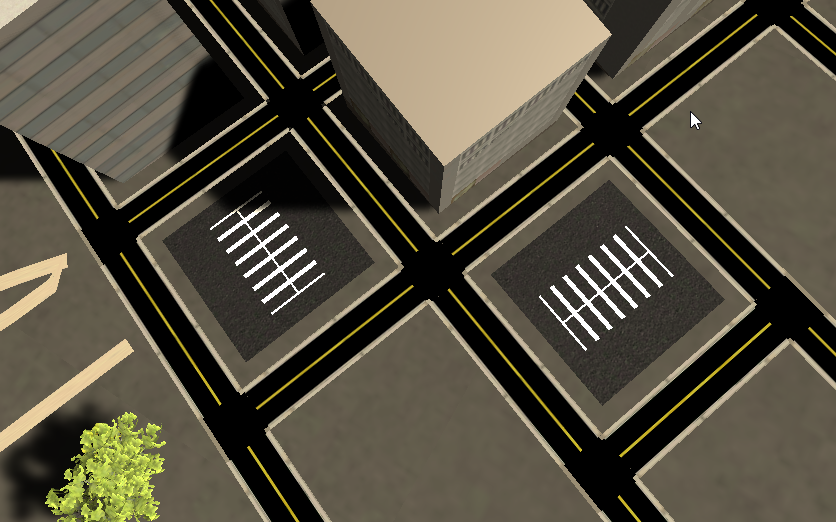
\includegraphics[width=\textwidth]{figure/results/parking/smallplots}}
     \caption{Two small parking lots consisting of one row.}
   \end{subfigure}
     \caption{Two examples of different sized parking lots created by the generator.}
   \label{fig:results_parking_sizebased}
 \end{figure}

These parking lots are generated by approximating the largest possible rectangle that fits inside a given plot, and then generating parking lots inside of it.
The number of rows is based on the size of the computed rectangle, and the algorithm aims to fit as many rows of parking lots inside the rectangle such that there still exists space between the rows for cars to enter.

Having the parking lots consist of multiple rows depending on the size gives some more variety, but the decision to do this was also based on real-world parking lots (see Figure~\ref{fig:parkings}).
In the left example in Figure~\ref{fig:parkings}, a road is used to separate parking spaces, making it impossible for parked cars to be surrounded and stuck by other parked cars.
The right example, however, has a more interesting shape, the parking lot in the center of it is shaped in the two-row style, while the surrounding rectangle is large enough that cars can easily drive around and not be blocked by parked cars.
This type of parking space is difficult to generate reliably in arbitrary plot shapes, consequently shapes like these were left out of the scope for this project.
